\documentclass[1p]{elsarticle_modified}
%\bibliographystyle{elsarticle-num}

%\usepackage[colorlinks]{hyperref}
%\usepackage{abbrmath_seonhwa} %\Abb, \Ascr, \Acal ,\Abf, \Afrak
\usepackage{amsfonts}
\usepackage{amssymb}
\usepackage{amsmath}
\usepackage{amsthm}
\usepackage{scalefnt}
\usepackage{amsbsy}
\usepackage{kotex}
\usepackage{caption}
\usepackage{subfig}
\usepackage{color}
\usepackage{graphicx}
\usepackage{xcolor} %% white, black, red, green, blue, cyan, magenta, yellow
\usepackage{float}
\usepackage{setspace}
\usepackage{hyperref}

\usepackage{tikz}
\usetikzlibrary{arrows}

\usepackage{multirow}
\usepackage{array} % fixed length table
\usepackage{hhline}

%%%%%%%%%%%%%%%%%%%%%
\makeatletter
\renewcommand*\env@matrix[1][\arraystretch]{%
	\edef\arraystretch{#1}%
	\hskip -\arraycolsep
	\let\@ifnextchar\new@ifnextchar
	\array{*\c@MaxMatrixCols c}}
\makeatother %https://tex.stackexchange.com/questions/14071/how-can-i-increase-the-line-spacing-in-a-matrix
%%%%%%%%%%%%%%%

\usepackage[normalem]{ulem}

\newcommand{\msout}[1]{\ifmmode\text{\sout{\ensuremath{#1}}}\else\sout{#1}\fi}
%SOURCE: \msout is \stkout macro in https://tex.stackexchange.com/questions/20609/strikeout-in-math-mode

\newcommand{\cancel}[1]{
	\ifmmode
	{\color{red}\msout{#1}}
	\else
	{\color{red}\sout{#1}}
	\fi
}

\newcommand{\add}[1]{
	{\color{blue}\uwave{#1}}
}

\newcommand{\replace}[2]{
	\ifmmode
	{\color{red}\msout{#1}}{\color{blue}\uwave{#2}}
	\else
	{\color{red}\sout{#1}}{\color{blue}\uwave{#2}}
	\fi
}

\newcommand{\Sol}{\mathcal{S}} %segment
\newcommand{\D}{D} %diagram
\newcommand{\A}{\mathcal{A}} %arc


%%%%%%%%%%%%%%%%%%%%%%%%%%%%%5 test

\def\sl{\operatorname{\textup{SL}}(2,\Cbb)}
\def\psl{\operatorname{\textup{PSL}}(2,\Cbb)}
\def\quan{\mkern 1mu \triangleright \mkern 1mu}

\theoremstyle{definition}
\newtheorem{thm}{Theorem}[section]
\newtheorem{prop}[thm]{Proposition}
\newtheorem{lem}[thm]{Lemma}
\newtheorem{ques}[thm]{Question}
\newtheorem{cor}[thm]{Corollary}
\newtheorem{defn}[thm]{Definition}
\newtheorem{exam}[thm]{Example}
\newtheorem{rmk}[thm]{Remark}
\newtheorem{alg}[thm]{Algorithm}

\newcommand{\I}{\sqrt{-1}}
\begin{document}

%\begin{frontmatter}
%
%\title{Boundary parabolic representations of knots up to 8 crossings}
%
%%% Group authors per affiliation:
%\author{Yunhi Cho} 
%\address{Department of Mathematics, University of Seoul, Seoul, Korea}
%\ead{yhcho@uos.ac.kr}
%
%
%\author{Seonhwa Kim} %\fnref{s_kim}}
%\address{Center for Geometry and Physics, Institute for Basic Science, Pohang, 37673, Korea}
%\ead{ryeona17@ibs.re.kr}
%
%\author{Hyuk Kim}
%\address{Department of Mathematical Sciences, Seoul National University, Seoul 08826, Korea}
%\ead{hyukkim@snu.ac.kr}
%
%\author{Seokbeom Yoon}
%\address{Department of Mathematical Sciences, Seoul National University, Seoul, 08826,  Korea}
%\ead{sbyoon15@snu.ac.kr}
%
%\begin{abstract}
%We find all boundary parabolic representation of knots up to 8 crossings.
%
%\end{abstract}
%\begin{keyword}
%    \MSC[2010] 57M25 
%\end{keyword}
%
%\end{frontmatter}

%\linenumbers
%\tableofcontents
%
\newcommand\colored[1]{\textcolor{white}{\rule[-0.35ex]{0.8em}{1.4ex}}\kern-0.8em\color{red} #1}%
%\newcommand\colored[1]{\textcolor{white}{ #1}\kern-2.17ex	\textcolor{white}{ #1}\kern-1.81ex	\textcolor{white}{ #1}\kern-2.15ex\color{red}#1	}

{\Large $\underline{11a_{201}~(K11a_{201})}$}

\setlength{\tabcolsep}{10pt}
\renewcommand{\arraystretch}{1.6}
\vspace{1cm}\begin{tabular}{m{100pt}>{\centering\arraybackslash}m{274pt}}
\multirow{5}{120pt}{
	\centering
	\includegraphics[width=112pt]{../../../GIT/diagram.site/Diagrams/png/450_11a_201.png}\\
\ \ \ A knot diagram\footnotemark}&
\allowdisplaybreaks
\textbf{Linearized knot diagam} \\
\cline{2-2}
 &
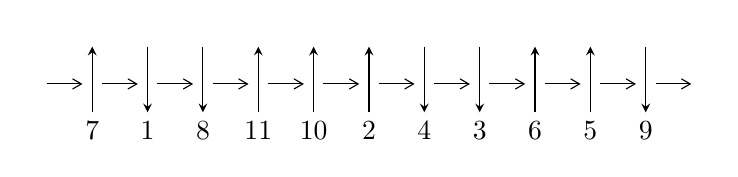
\begin{tikzpicture}[x=20pt, y=17pt]
	% nodes
	\node (C0) at (0, 0) {};
	\node (C1) at (1, 0) {};
	\node (C1U) at (1, +1) {};
	\node (C1D) at (1, -1) {7};

	\node (C2) at (2, 0) {};
	\node (C2U) at (2, +1) {};
	\node (C2D) at (2, -1) {1};

	\node (C3) at (3, 0) {};
	\node (C3U) at (3, +1) {};
	\node (C3D) at (3, -1) {8};

	\node (C4) at (4, 0) {};
	\node (C4U) at (4, +1) {};
	\node (C4D) at (4, -1) {11};

	\node (C5) at (5, 0) {};
	\node (C5U) at (5, +1) {};
	\node (C5D) at (5, -1) {10};

	\node (C6) at (6, 0) {};
	\node (C6U) at (6, +1) {};
	\node (C6D) at (6, -1) {2};

	\node (C7) at (7, 0) {};
	\node (C7U) at (7, +1) {};
	\node (C7D) at (7, -1) {4};

	\node (C8) at (8, 0) {};
	\node (C8U) at (8, +1) {};
	\node (C8D) at (8, -1) {3};

	\node (C9) at (9, 0) {};
	\node (C9U) at (9, +1) {};
	\node (C9D) at (9, -1) {6};

	\node (C10) at (10, 0) {};
	\node (C10U) at (10, +1) {};
	\node (C10D) at (10, -1) {5};

	\node (C11) at (11, 0) {};
	\node (C11U) at (11, +1) {};
	\node (C11D) at (11, -1) {9};
	\node (C12) at (12, 0) {};

	% arrows
	\draw[->,>={angle 60}]
	(C0) edge (C1) (C1) edge (C2) (C2) edge (C3) (C3) edge (C4) (C4) edge (C5) (C5) edge (C6) (C6) edge (C7) (C7) edge (C8) (C8) edge (C9) (C9) edge (C10) (C10) edge (C11) (C11) edge (C12) ;	\draw[->,>=stealth]
	(C1D) edge (C1U) (C2U) edge (C2D) (C3U) edge (C3D) (C4D) edge (C4U) (C5D) edge (C5U) (C6D) edge (C6U) (C7U) edge (C7D) (C8U) edge (C8D) (C9D) edge (C9U) (C10D) edge (C10U) (C11U) edge (C11D) ;
	\end{tikzpicture} \\
\hhline{~~} \\& 
\textbf{Solving Sequence} \\ \cline{2-2} 
 &
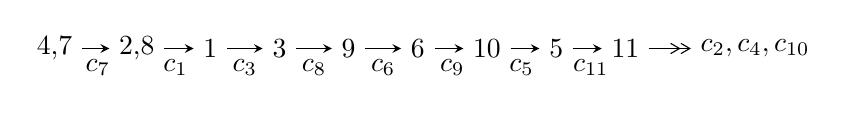
\begin{tikzpicture}[x=25pt, y=7pt]
	% node
	\node (A0) at (-1/8, 0) {4,7};
	\node (A1) at (17/16, 0) {2,8};
	\node (A2) at (17/8, 0) {1};
	\node (A3) at (25/8, 0) {3};
	\node (A4) at (33/8, 0) {9};
	\node (A5) at (41/8, 0) {6};
	\node (A6) at (49/8, 0) {10};
	\node (A7) at (57/8, 0) {5};
	\node (A8) at (65/8, 0) {11};
	\node (C1) at (1/2, -1) {$c_{7}$};
	\node (C2) at (13/8, -1) {$c_{1}$};
	\node (C3) at (21/8, -1) {$c_{3}$};
	\node (C4) at (29/8, -1) {$c_{8}$};
	\node (C5) at (37/8, -1) {$c_{6}$};
	\node (C6) at (45/8, -1) {$c_{9}$};
	\node (C7) at (53/8, -1) {$c_{5}$};
	\node (C8) at (61/8, -1) {$c_{11}$};
	\node (A9) at (10, 0) {$c_{2},c_{4},c_{10}$};

	% edge
	\draw[->,>=stealth]	
	(A0) edge (A1) (A1) edge (A2) (A2) edge (A3) (A3) edge (A4) (A4) edge (A5) (A5) edge (A6) (A6) edge (A7) (A7) edge (A8) ;
	\draw[->>,>={angle 60}]	
	(A8) edge (A9);
\end{tikzpicture} \\ 

\end{tabular} \\

\footnotetext{
The image of knot diagram is generated by the software ``\textbf{Draw programme}" developed by Andrew Bartholomew(\url{http://www.layer8.co.uk/maths/draw/index.htm\#Running-draw}), where we modified some parts for our purpose(\url{https://github.com/CATsTAILs/LinksPainter}).
}\phantom \\ \newline 
\centering \textbf{Ideals for irreducible components\footnotemark of $X_{\text{par}}$} 
 
\begin{align*}
I^u_{1}&=\langle 
4375317 u^{31}-2433496 u^{30}+\cdots+41310281 b+29259312,\\
\phantom{I^u_{1}}&\phantom{= \langle  }497615779 u^{31}+479325734 u^{30}+\cdots+826205620 a+3336436539,\;u^{32}+u^{31}+\cdots+6 u+5\rangle \\
I^u_{2}&=\langle 
b- u,\;a- u,\;u^{12}+4 u^{10}- u^9+6 u^8-3 u^7+5 u^6-3 u^5+3 u^4- u^3+u^2+1\rangle \\
I^u_{3}&=\langle 
b- u,\;a^2-2 a u+a- u-2,\;u^2+1\rangle \\
\\
\end{align*}
\raggedright * 3 irreducible components of $\dim_{\mathbb{C}}=0$, with total 48 representations.\\
\footnotetext{All coefficients of polynomials are rational numbers. But the coefficients are sometimes approximated in decimal forms when there is not enough margin.}
\newpage
\renewcommand{\arraystretch}{1}
\centering \section*{I. $I^u_{1}= \langle 4.38\times10^{6} u^{31}-2.43\times10^{6} u^{30}+\cdots+4.13\times10^{7} b+2.93\times10^{7},\;4.98\times10^{8} u^{31}+4.79\times10^{8} u^{30}+\cdots+8.26\times10^{8} a+3.34\times10^{9},\;u^{32}+u^{31}+\cdots+6 u+5 \rangle$}
\flushleft \textbf{(i) Arc colorings}\\
\begin{tabular}{m{7pt} m{180pt} m{7pt} m{180pt} }
\flushright $a_{4}=$&$\begin{pmatrix}0\\u\end{pmatrix}$ \\
\flushright $a_{7}=$&$\begin{pmatrix}1\\0\end{pmatrix}$ \\
\flushright $a_{2}=$&$\begin{pmatrix}-0.602290 u^{31}-0.580153 u^{30}+\cdots+1.15611 u-4.03826\\-0.105914 u^{31}+0.0589078 u^{30}+\cdots+0.0313659 u-0.708282\end{pmatrix}$ \\
\flushright $a_{8}=$&$\begin{pmatrix}1\\u^2\end{pmatrix}$ \\
\flushright $a_{1}=$&$\begin{pmatrix}-0.496377 u^{31}-0.639061 u^{30}+\cdots+1.12474 u-3.32998\\-0.105914 u^{31}+0.0589078 u^{30}+\cdots+0.0313659 u-0.708282\end{pmatrix}$ \\
\flushright $a_{3}=$&$\begin{pmatrix}u\\u^3+u\end{pmatrix}$ \\
\flushright $a_{9}=$&$\begin{pmatrix}u^2+1\\u^4+2 u^2\end{pmatrix}$ \\
\flushright $a_{6}=$&$\begin{pmatrix}0.119519 u^{31}-0.242713 u^{30}+\cdots-1.19552 u-3.13015\\-0.164821 u^{31}-0.336590 u^{30}+\cdots+0.0728005 u-1.52957\end{pmatrix}$ \\
\flushright $a_{10}=$&$\begin{pmatrix}-0.674669 u^{31}-0.189419 u^{30}+\cdots+2.00688 u-3.69475\\-0.0228362 u^{31}-0.319476 u^{30}+\cdots-0.115047 u-2.13688\end{pmatrix}$ \\
\flushright $a_{5}=$&$\begin{pmatrix}0.479860 u^{31}+0.593758 u^{30}+\cdots-4.21292 u+4.09540\\0.222814 u^{31}-0.00541149 u^{30}+\cdots-3.26130 u+2.60177\end{pmatrix}$ \\
\flushright $a_{11}=$&$\begin{pmatrix}-0.216037 u^{31}-0.00644846 u^{30}+\cdots+0.896572 u-2.42097\\0.216748 u^{31}+0.489956 u^{30}+\cdots+0.135123 u-0.963031\end{pmatrix}$\\ \flushright $a_{11}=$&$\begin{pmatrix}-0.216037 u^{31}-0.00644846 u^{30}+\cdots+0.896572 u-2.42097\\0.216748 u^{31}+0.489956 u^{30}+\cdots+0.135123 u-0.963031\end{pmatrix}$\\&\end{tabular}
\flushleft \textbf{(ii) Obstruction class $= -1$}\\~\\
\flushleft \textbf{(iii) Cusp Shapes $= \frac{5988531}{41310281} u^{31}-\frac{30382789}{41310281} u^{30}+\cdots-\frac{272513748}{41310281} u-\frac{494571835}{41310281}$}\\~\\
\newpage\renewcommand{\arraystretch}{1}
\flushleft \textbf{(iv) u-Polynomials at the component}\newline \\
\begin{tabular}{m{50pt}|m{274pt}}
Crossings & \hspace{64pt}u-Polynomials at each crossing \\
\hline $$\begin{aligned}c_{1},c_{6}\end{aligned}$$&$\begin{aligned}
&u^{32}+u^{31}+\cdots+4 u+5
\end{aligned}$\\
\hline $$\begin{aligned}c_{2}\end{aligned}$$&$\begin{aligned}
&u^{32}+13 u^{31}+\cdots+274 u+25
\end{aligned}$\\
\hline $$\begin{aligned}c_{3},c_{7},c_{8}\end{aligned}$$&$\begin{aligned}
&u^{32}+u^{31}+\cdots+6 u+5
\end{aligned}$\\
\hline $$\begin{aligned}c_{4},c_{5},c_{9}\\c_{10}\end{aligned}$$&$\begin{aligned}
&u^{32}+2 u^{31}+\cdots+5 u+2
\end{aligned}$\\
\hline $$\begin{aligned}c_{11}\end{aligned}$$&$\begin{aligned}
&u^{32}-8 u^{31}+\cdots-91 u+136
\end{aligned}$\\
\hline
\end{tabular}\\~\\
\newpage\renewcommand{\arraystretch}{1}
\flushleft \textbf{(v) Riley Polynomials at the component}\newline \\
\begin{tabular}{m{50pt}|m{274pt}}
Crossings & \hspace{64pt}Riley Polynomials at each crossing \\
\hline $$\begin{aligned}c_{1},c_{6}\end{aligned}$$&$\begin{aligned}
&y^{32}+13 y^{31}+\cdots+274 y+25
\end{aligned}$\\
\hline $$\begin{aligned}c_{2}\end{aligned}$$&$\begin{aligned}
&y^{32}+17 y^{31}+\cdots+3174 y+625
\end{aligned}$\\
\hline $$\begin{aligned}c_{3},c_{7},c_{8}\end{aligned}$$&$\begin{aligned}
&y^{32}+33 y^{31}+\cdots-206 y+25
\end{aligned}$\\
\hline $$\begin{aligned}c_{4},c_{5},c_{9}\\c_{10}\end{aligned}$$&$\begin{aligned}
&y^{32}+36 y^{31}+\cdots+19 y+4
\end{aligned}$\\
\hline $$\begin{aligned}c_{11}\end{aligned}$$&$\begin{aligned}
&y^{32}+8 y^{30}+\cdots+159543 y+18496
\end{aligned}$\\
\hline
\end{tabular}\\~\\
\newpage\flushleft \textbf{(vi) Complex Volumes and Cusp Shapes}
$$\begin{array}{c|c|c}  
\text{Solutions to }I^u_{1}& \I (\text{vol} + \sqrt{-1}CS) & \text{Cusp shape}\\
 \hline 
\begin{aligned}
u &= \phantom{-}0.551100 + 0.734939 I \\
a &= \phantom{-}0.107390 + 1.226730 I \\
b &= -0.591788 + 0.593098 I\end{aligned}
 & -5.67221 - 1.34508 I & -0.32319 + 3.71865 I \\ \hline\begin{aligned}
u &= \phantom{-}0.551100 - 0.734939 I \\
a &= \phantom{-}0.107390 - 1.226730 I \\
b &= -0.591788 - 0.593098 I\end{aligned}
 & -5.67221 + 1.34508 I & -0.32319 - 3.71865 I \\ \hline\begin{aligned}
u &= -0.875527 + 0.268870 I \\
a &= -0.16524 + 2.17598 I \\
b &= \phantom{-}0.579991 + 1.106900 I\end{aligned}
 & -8.94868 + 8.17553 I & -4.60823 - 6.25670 I \\ \hline\begin{aligned}
u &= -0.875527 - 0.268870 I \\
a &= -0.16524 - 2.17598 I \\
b &= \phantom{-}0.579991 - 1.106900 I\end{aligned}
 & -8.94868 - 8.17553 I & -4.60823 + 6.25670 I \\ \hline\begin{aligned}
u &= \phantom{-}0.784850 + 0.315450 I \\
a &= \phantom{-}0.29529 + 2.03118 I \\
b &= -0.548702 + 1.030460 I\end{aligned}
 & -1.40224 - 5.85456 I & -1.92239 + 8.44410 I \\ \hline\begin{aligned}
u &= \phantom{-}0.784850 - 0.315450 I \\
a &= \phantom{-}0.29529 - 2.03118 I \\
b &= -0.548702 - 1.030460 I\end{aligned}
 & -1.40224 + 5.85456 I & -1.92239 - 8.44410 I \\ \hline\begin{aligned}
u &= -0.638976 + 0.376897 I \\
a &= -0.49487 + 1.75535 I \\
b &= \phantom{-}0.482595 + 0.918929 I\end{aligned}
 & -0.22348 + 2.37773 I & \phantom{-}1.52399 - 3.08946 I \\ \hline\begin{aligned}
u &= -0.638976 - 0.376897 I \\
a &= -0.49487 - 1.75535 I \\
b &= \phantom{-}0.482595 - 0.918929 I\end{aligned}
 & -0.22348 - 2.37773 I & \phantom{-}1.52399 + 3.08946 I \\ \hline\begin{aligned}
u &= -0.135432 + 1.257600 I \\
a &= \phantom{-}1.98986 - 0.02746 I \\
b &= -0.422506 - 0.889378 I\end{aligned}
 & -7.83825 + 1.73312 I & -0.29629 - 4.34437 I \\ \hline\begin{aligned}
u &= -0.135432 - 1.257600 I \\
a &= \phantom{-}1.98986 + 0.02746 I \\
b &= -0.422506 + 0.889378 I\end{aligned}
 & -7.83825 - 1.73312 I & -0.29629 + 4.34437 I\\
 \hline 
 \end{array}$$\newpage$$\begin{array}{c|c|c}  
\text{Solutions to }I^u_{1}& \I (\text{vol} + \sqrt{-1}CS) & \text{Cusp shape}\\
 \hline 
\begin{aligned}
u &= -0.170928 + 0.653284 I \\
a &= -0.210272 + 0.793110 I \\
b &= \phantom{-}0.184737 + 0.516971 I\end{aligned}
 & \phantom{-}0.317055 + 1.041090 I & \phantom{-}4.08687 - 7.01179 I \\ \hline\begin{aligned}
u &= -0.170928 - 0.653284 I \\
a &= -0.210272 - 0.793110 I \\
b &= \phantom{-}0.184737 - 0.516971 I\end{aligned}
 & \phantom{-}0.317055 - 1.041090 I & \phantom{-}4.08687 + 7.01179 I \\ \hline\begin{aligned}
u &= \phantom{-}0.138560 + 1.382420 I \\
a &= -1.208030 - 0.407595 I \\
b &= \phantom{-}0.611494 - 0.902238 I\end{aligned}
 & \phantom{-}1.47357 - 2.48254 I & \phantom{-}0.77846 + 2.31990 I \\ \hline\begin{aligned}
u &= \phantom{-}0.138560 - 1.382420 I \\
a &= -1.208030 + 0.407595 I \\
b &= \phantom{-}0.611494 + 0.902238 I\end{aligned}
 & \phantom{-}1.47357 + 2.48254 I & \phantom{-}0.77846 - 2.31990 I \\ \hline\begin{aligned}
u &= \phantom{-}0.11167 + 1.45794 I \\
a &= \phantom{-}0.322969 + 0.098145 I \\
b &= -0.836425 - 0.572540 I\end{aligned}
 & \phantom{-}7.07545 + 0.03254 I & \phantom{-}6.68754 - 2.41599 I \\ \hline\begin{aligned}
u &= \phantom{-}0.11167 - 1.45794 I \\
a &= \phantom{-}0.322969 - 0.098145 I \\
b &= -0.836425 + 0.572540 I\end{aligned}
 & \phantom{-}7.07545 - 0.03254 I & \phantom{-}6.68754 + 2.41599 I \\ \hline\begin{aligned}
u &= -0.19688 + 1.45123 I \\
a &= -0.142970 + 0.223499 I \\
b &= \phantom{-}0.888417 - 0.454350 I\end{aligned}
 & \phantom{-}6.27640 + 4.08548 I & \phantom{-}4.92629 - 3.95232 I \\ \hline\begin{aligned}
u &= -0.19688 - 1.45123 I \\
a &= -0.142970 - 0.223499 I \\
b &= \phantom{-}0.888417 + 0.454350 I\end{aligned}
 & \phantom{-}6.27640 - 4.08548 I & \phantom{-}4.92629 + 3.95232 I \\ \hline\begin{aligned}
u &= -0.23997 + 1.44565 I \\
a &= \phantom{-}1.055980 - 0.926944 I \\
b &= -0.674652 - 1.050250 I\end{aligned}
 & \phantom{-}5.62992 + 5.59260 I & \phantom{-}4.88199 - 3.14064 I \\ \hline\begin{aligned}
u &= -0.23997 - 1.44565 I \\
a &= \phantom{-}1.055980 + 0.926944 I \\
b &= -0.674652 + 1.050250 I\end{aligned}
 & \phantom{-}5.62992 - 5.59260 I & \phantom{-}4.88199 + 3.14064 I\\
 \hline 
 \end{array}$$\newpage$$\begin{array}{c|c|c}  
\text{Solutions to }I^u_{1}& \I (\text{vol} + \sqrt{-1}CS) & \text{Cusp shape}\\
 \hline 
\begin{aligned}
u &= -0.518541 + 0.098182 I \\
a &= -1.13760 - 3.26930 I \\
b &= \phantom{-}0.224351 - 1.142550 I\end{aligned}
 & -11.37260 + 0.54600 I & -8.69124 + 0.03376 I \\ \hline\begin{aligned}
u &= -0.518541 - 0.098182 I \\
a &= -1.13760 + 3.26930 I \\
b &= \phantom{-}0.224351 + 1.142550 I\end{aligned}
 & -11.37260 - 0.54600 I & -8.69124 - 0.03376 I \\ \hline\begin{aligned}
u &= \phantom{-}0.27546 + 1.44706 I \\
a &= -0.003952 + 0.310620 I \\
b &= -0.944505 - 0.352972 I\end{aligned}
 & -0.98639 - 6.83283 I & \phantom{-}1.75203 + 3.32072 I \\ \hline\begin{aligned}
u &= \phantom{-}0.27546 - 1.44706 I \\
a &= -0.003952 - 0.310620 I \\
b &= -0.944505 + 0.352972 I\end{aligned}
 & -0.98639 + 6.83283 I & \phantom{-}1.75203 - 3.32072 I \\ \hline\begin{aligned}
u &= \phantom{-}0.02294 + 1.47346 I \\
a &= -0.614412 - 0.215049 I \\
b &= \phantom{-}0.781589 - 0.768693 I\end{aligned}
 & \phantom{-}1.77631 - 2.78949 I & \phantom{-}2.31170 + 3.04495 I \\ \hline\begin{aligned}
u &= \phantom{-}0.02294 - 1.47346 I \\
a &= -0.614412 + 0.215049 I \\
b &= \phantom{-}0.781589 + 0.768693 I\end{aligned}
 & \phantom{-}1.77631 + 2.78949 I & \phantom{-}2.31170 - 3.04495 I \\ \hline\begin{aligned}
u &= \phantom{-}0.30286 + 1.44432 I \\
a &= -1.07271 - 1.17133 I \\
b &= \phantom{-}0.660399 - 1.126280 I\end{aligned}
 & \phantom{-}4.24750 - 9.79490 I & \phantom{-}1.90027 + 8.12544 I \\ \hline\begin{aligned}
u &= \phantom{-}0.30286 - 1.44432 I \\
a &= -1.07271 + 1.17133 I \\
b &= \phantom{-}0.660399 + 1.126280 I\end{aligned}
 & \phantom{-}4.24750 + 9.79490 I & \phantom{-}1.90027 - 8.12544 I \\ \hline\begin{aligned}
u &= -0.35408 + 1.43602 I \\
a &= \phantom{-}1.08498 - 1.36239 I \\
b &= -0.641332 - 1.184000 I\end{aligned}
 & -3.50806 + 12.60760 I & -1.01142 - 7.01526 I \\ \hline\begin{aligned}
u &= -0.35408 - 1.43602 I \\
a &= \phantom{-}1.08498 + 1.36239 I \\
b &= -0.641332 + 1.184000 I\end{aligned}
 & -3.50806 - 12.60760 I & -1.01142 + 7.01526 I\\
 \hline 
 \end{array}$$\newpage$$\begin{array}{c|c|c}  
\text{Solutions to }I^u_{1}& \I (\text{vol} + \sqrt{-1}CS) & \text{Cusp shape}\\
 \hline 
\begin{aligned}
u &= \phantom{-}0.442891 + 0.103566 I \\
a &= \phantom{-}1.59360 + 2.25219 I \\
b &= -0.253664 + 1.015980 I\end{aligned}
 & -3.29365 - 0.43865 I & -7.99639 - 0.07898 I \\ \hline\begin{aligned}
u &= \phantom{-}0.442891 - 0.103566 I \\
a &= \phantom{-}1.59360 - 2.25219 I \\
b &= -0.253664 - 1.015980 I\end{aligned}
 & -3.29365 + 0.43865 I & -7.99639 + 0.07898 I\\
 \hline 
 \end{array}$$\newpage\newpage\renewcommand{\arraystretch}{1}
\centering \section*{II. $I^u_{2}= \langle b- u,\;a- u,\;u^{12}+4 u^{10}+\cdots+u^2+1 \rangle$}
\flushleft \textbf{(i) Arc colorings}\\
\begin{tabular}{m{7pt} m{180pt} m{7pt} m{180pt} }
\flushright $a_{4}=$&$\begin{pmatrix}0\\u\end{pmatrix}$ \\
\flushright $a_{7}=$&$\begin{pmatrix}1\\0\end{pmatrix}$ \\
\flushright $a_{2}=$&$\begin{pmatrix}u\\u\end{pmatrix}$ \\
\flushright $a_{8}=$&$\begin{pmatrix}1\\u^2\end{pmatrix}$ \\
\flushright $a_{1}=$&$\begin{pmatrix}0\\u\end{pmatrix}$ \\
\flushright $a_{3}=$&$\begin{pmatrix}u\\u^3+u\end{pmatrix}$ \\
\flushright $a_{9}=$&$\begin{pmatrix}u^2+1\\u^4+2 u^2\end{pmatrix}$ \\
\flushright $a_{6}=$&$\begin{pmatrix}u^2+1\\u^2\end{pmatrix}$ \\
\flushright $a_{10}=$&$\begin{pmatrix}u^8+3 u^6+3 u^4+2 u^2+1\\u^8+2 u^6+2 u^4+2 u^2\end{pmatrix}$ \\
\flushright $a_{5}=$&$\begin{pmatrix}u^{11}+4 u^9+6 u^7+4 u^5+u^3\\u^{11}+u^{10}+3 u^9+3 u^8+3 u^7+3 u^6+u^5+u^4\end{pmatrix}$ \\
\flushright $a_{11}=$&$\begin{pmatrix}u^5+2 u^3+u\\u^7+3 u^5+2 u^3+u\end{pmatrix}$\\ \flushright $a_{11}=$&$\begin{pmatrix}u^5+2 u^3+u\\u^7+3 u^5+2 u^3+u\end{pmatrix}$\\&\end{tabular}
\flushleft \textbf{(ii) Obstruction class $= -1$}\\~\\
\flushleft \textbf{(iii) Cusp Shapes $= 4 u^6+8 u^4-4 u^3+4 u^2-4 u+2$}\\~\\
\newpage\renewcommand{\arraystretch}{1}
\flushleft \textbf{(iv) u-Polynomials at the component}\newline \\
\begin{tabular}{m{50pt}|m{274pt}}
Crossings & \hspace{64pt}u-Polynomials at each crossing \\
\hline $$\begin{aligned}c_{1},c_{3},c_{6}\\c_{7},c_{8}\end{aligned}$$&$\begin{aligned}
&u^{12}+4 u^{10}- u^9+6 u^8-3 u^7+5 u^6-3 u^5+3 u^4- u^3+u^2+1
\end{aligned}$\\
\hline $$\begin{aligned}c_{2}\end{aligned}$$&$\begin{aligned}
&u^{12}+8 u^{11}+\cdots+2 u+1
\end{aligned}$\\
\hline $$\begin{aligned}c_{4},c_{5},c_{9}\\c_{10}\end{aligned}$$&$\begin{aligned}
&(u^4- u^3+3 u^2-2 u+1)^3
\end{aligned}$\\
\hline $$\begin{aligned}c_{11}\end{aligned}$$&$\begin{aligned}
&(u^4- u^3+u^2+1)^3
\end{aligned}$\\
\hline
\end{tabular}\\~\\
\newpage\renewcommand{\arraystretch}{1}
\flushleft \textbf{(v) Riley Polynomials at the component}\newline \\
\begin{tabular}{m{50pt}|m{274pt}}
Crossings & \hspace{64pt}Riley Polynomials at each crossing \\
\hline $$\begin{aligned}c_{1},c_{3},c_{6}\\c_{7},c_{8}\end{aligned}$$&$\begin{aligned}
&y^{12}+8 y^{11}+\cdots+2 y+1
\end{aligned}$\\
\hline $$\begin{aligned}c_{2}\end{aligned}$$&$\begin{aligned}
&y^{12}-8 y^{11}+\cdots+10 y+1
\end{aligned}$\\
\hline $$\begin{aligned}c_{4},c_{5},c_{9}\\c_{10}\end{aligned}$$&$\begin{aligned}
&(y^4+5 y^3+7 y^2+2 y+1)^3
\end{aligned}$\\
\hline $$\begin{aligned}c_{11}\end{aligned}$$&$\begin{aligned}
&(y^4+y^3+3 y^2+2 y+1)^3
\end{aligned}$\\
\hline
\end{tabular}\\~\\
\newpage\flushleft \textbf{(vi) Complex Volumes and Cusp Shapes}
$$\begin{array}{c|c|c}  
\text{Solutions to }I^u_{2}& \I (\text{vol} + \sqrt{-1}CS) & \text{Cusp shape}\\
 \hline 
\begin{aligned}
u &= \phantom{-}0.427976 + 0.817556 I \\
a &= \phantom{-}0.427976 + 0.817556 I \\
b &= \phantom{-}0.427976 + 0.817556 I\end{aligned}
 & \phantom{-}0.21101 + 1.41510 I & \phantom{-}1.82674 - 4.90874 I \\ \hline\begin{aligned}
u &= \phantom{-}0.427976 - 0.817556 I \\
a &= \phantom{-}0.427976 - 0.817556 I \\
b &= \phantom{-}0.427976 - 0.817556 I\end{aligned}
 & \phantom{-}0.21101 - 1.41510 I & \phantom{-}1.82674 + 4.90874 I \\ \hline\begin{aligned}
u &= -0.543763 + 0.976761 I \\
a &= -0.543763 + 0.976761 I \\
b &= -0.543763 + 0.976761 I\end{aligned}
 & -6.79074 - 3.16396 I & -1.82674 + 2.56480 I \\ \hline\begin{aligned}
u &= -0.543763 - 0.976761 I \\
a &= -0.543763 - 0.976761 I \\
b &= -0.543763 - 0.976761 I\end{aligned}
 & -6.79074 + 3.16396 I & -1.82674 - 2.56480 I \\ \hline\begin{aligned}
u &= \phantom{-}0.739694 + 0.363125 I \\
a &= \phantom{-}0.739694 + 0.363125 I \\
b &= \phantom{-}0.739694 + 0.363125 I\end{aligned}
 & -6.79074 - 3.16396 I & -1.82674 + 2.56480 I \\ \hline\begin{aligned}
u &= \phantom{-}0.739694 - 0.363125 I \\
a &= \phantom{-}0.739694 - 0.363125 I \\
b &= \phantom{-}0.739694 - 0.363125 I\end{aligned}
 & -6.79074 + 3.16396 I & -1.82674 - 2.56480 I \\ \hline\begin{aligned}
u &= \phantom{-}0.093076 + 1.263390 I \\
a &= \phantom{-}0.093076 + 1.263390 I \\
b &= \phantom{-}0.093076 + 1.263390 I\end{aligned}
 & \phantom{-}0.21101 - 1.41510 I & \phantom{-}1.82674 + 4.90874 I \\ \hline\begin{aligned}
u &= \phantom{-}0.093076 - 1.263390 I \\
a &= \phantom{-}0.093076 - 1.263390 I \\
b &= \phantom{-}0.093076 - 1.263390 I\end{aligned}
 & \phantom{-}0.21101 + 1.41510 I & \phantom{-}1.82674 - 4.90874 I \\ \hline\begin{aligned}
u &= -0.521051 + 0.445835 I \\
a &= -0.521051 + 0.445835 I \\
b &= -0.521051 + 0.445835 I\end{aligned}
 & \phantom{-}0.21101 + 1.41510 I & \phantom{-}1.82674 - 4.90874 I \\ \hline\begin{aligned}
u &= -0.521051 - 0.445835 I \\
a &= -0.521051 - 0.445835 I \\
b &= -0.521051 - 0.445835 I\end{aligned}
 & \phantom{-}0.21101 - 1.41510 I & \phantom{-}1.82674 + 4.90874 I\\
 \hline 
 \end{array}$$\newpage$$\begin{array}{c|c|c}  
\text{Solutions to }I^u_{2}& \I (\text{vol} + \sqrt{-1}CS) & \text{Cusp shape}\\
 \hline 
\begin{aligned}
u &= -0.195931 + 1.339890 I \\
a &= -0.195931 + 1.339890 I \\
b &= -0.195931 + 1.339890 I\end{aligned}
 & -6.79074 + 3.16396 I & -1.82674 - 2.56480 I \\ \hline\begin{aligned}
u &= -0.195931 - 1.339890 I \\
a &= -0.195931 - 1.339890 I \\
b &= -0.195931 - 1.339890 I\end{aligned}
 & -6.79074 - 3.16396 I & -1.82674 + 2.56480 I\\
 \hline 
 \end{array}$$\newpage\newpage\renewcommand{\arraystretch}{1}
\centering \section*{III. $I^u_{3}= \langle b- u,\;a^2-2 a u+a- u-2,\;u^2+1 \rangle$}
\flushleft \textbf{(i) Arc colorings}\\
\begin{tabular}{m{7pt} m{180pt} m{7pt} m{180pt} }
\flushright $a_{4}=$&$\begin{pmatrix}0\\u\end{pmatrix}$ \\
\flushright $a_{7}=$&$\begin{pmatrix}1\\0\end{pmatrix}$ \\
\flushright $a_{2}=$&$\begin{pmatrix}a\\u\end{pmatrix}$ \\
\flushright $a_{8}=$&$\begin{pmatrix}1\\-1\end{pmatrix}$ \\
\flushright $a_{1}=$&$\begin{pmatrix}a- u\\u\end{pmatrix}$ \\
\flushright $a_{3}=$&$\begin{pmatrix}u\\0\end{pmatrix}$ \\
\flushright $a_{9}=$&$\begin{pmatrix}0\\-1\end{pmatrix}$ \\
\flushright $a_{6}=$&$\begin{pmatrix}a u+1\\-1\end{pmatrix}$ \\
\flushright $a_{10}=$&$\begin{pmatrix}- a+u+1\\a u\end{pmatrix}$ \\
\flushright $a_{5}=$&$\begin{pmatrix}- a u+u-1\\a u- a+u+1\end{pmatrix}$ \\
\flushright $a_{11}=$&$\begin{pmatrix}a- u\\- a+2 u\end{pmatrix}$\\ \flushright $a_{11}=$&$\begin{pmatrix}a- u\\- a+2 u\end{pmatrix}$\\&\end{tabular}
\flushleft \textbf{(ii) Obstruction class $= 1$}\\~\\
\flushleft \textbf{(iii) Cusp Shapes $= -4$}\\~\\
\newpage\renewcommand{\arraystretch}{1}
\flushleft \textbf{(iv) u-Polynomials at the component}\newline \\
\begin{tabular}{m{50pt}|m{274pt}}
Crossings & \hspace{64pt}u-Polynomials at each crossing \\
\hline $$\begin{aligned}c_{1},c_{3},c_{6}\\c_{7},c_{8}\end{aligned}$$&$\begin{aligned}
&(u^2+1)^2
\end{aligned}$\\
\hline $$\begin{aligned}c_{2}\end{aligned}$$&$\begin{aligned}
&(u+1)^4
\end{aligned}$\\
\hline $$\begin{aligned}c_{4},c_{5},c_{9}\\c_{10}\end{aligned}$$&$\begin{aligned}
&u^4+3 u^2+1
\end{aligned}$\\
\hline $$\begin{aligned}c_{11}\end{aligned}$$&$\begin{aligned}
&(u^2- u-1)^2
\end{aligned}$\\
\hline
\end{tabular}\\~\\
\newpage\renewcommand{\arraystretch}{1}
\flushleft \textbf{(v) Riley Polynomials at the component}\newline \\
\begin{tabular}{m{50pt}|m{274pt}}
Crossings & \hspace{64pt}Riley Polynomials at each crossing \\
\hline $$\begin{aligned}c_{1},c_{3},c_{6}\\c_{7},c_{8}\end{aligned}$$&$\begin{aligned}
&(y+1)^4
\end{aligned}$\\
\hline $$\begin{aligned}c_{2}\end{aligned}$$&$\begin{aligned}
&(y-1)^4
\end{aligned}$\\
\hline $$\begin{aligned}c_{4},c_{5},c_{9}\\c_{10}\end{aligned}$$&$\begin{aligned}
&(y^2+3 y+1)^2
\end{aligned}$\\
\hline $$\begin{aligned}c_{11}\end{aligned}$$&$\begin{aligned}
&(y^2-3 y+1)^2
\end{aligned}$\\
\hline
\end{tabular}\\~\\
\newpage\flushleft \textbf{(vi) Complex Volumes and Cusp Shapes}
$$\begin{array}{c|c|c}  
\text{Solutions to }I^u_{3}& \I (\text{vol} + \sqrt{-1}CS) & \text{Cusp shape}\\
 \hline 
\begin{aligned}
u &= \phantom{-0.000000 -}1.000000 I \\
a &= \phantom{-}0.618034 + 1.000000 I \\
b &= \phantom{-0.000000 -}1.000000 I\end{aligned}
 & -0.986960\phantom{ +0.000000I} & -4.00000\phantom{ +0.000000I} \\ \hline\begin{aligned}
u &= \phantom{-0.000000 -}1.000000 I \\
a &= -1.61803 + 1.00000 I \\
b &= \phantom{-0.000000 -}1.000000 I\end{aligned}
 & -8.88264\phantom{ +0.000000I} & -4.00000\phantom{ +0.000000I} \\ \hline\begin{aligned}
u &= \phantom{-0.000000 } -1.000000 I \\
a &= \phantom{-}0.618034 - 1.000000 I \\
b &= \phantom{-0.000000 } -1.000000 I\end{aligned}
 & -0.986960\phantom{ +0.000000I} & -4.00000\phantom{ +0.000000I} \\ \hline\begin{aligned}
u &= \phantom{-0.000000 } -1.000000 I \\
a &= -1.61803 - 1.00000 I \\
b &= \phantom{-0.000000 } -1.000000 I\end{aligned}
 & -8.88264\phantom{ +0.000000I} & -4.00000\phantom{ +0.000000I}\\
 \hline 
 \end{array}$$\newpage
\newpage\renewcommand{\arraystretch}{1}
\centering \section*{ IV. u-Polynomials}
\begin{tabular}{m{50pt}|m{274pt}}
Crossings & \hspace{64pt}u-Polynomials at each crossing \\
\hline $$\begin{aligned}c_{1},c_{6}\end{aligned}$$&$\begin{aligned}
&(u^2+1)^2(u^{12}+4 u^{10}- u^9+6 u^8-3 u^7+5 u^6-3 u^5+3 u^4- u^3+u^2+1)\\
&\cdot(u^{32}+u^{31}+\cdots+4 u+5)
\end{aligned}$\\
\hline $$\begin{aligned}c_{2}\end{aligned}$$&$\begin{aligned}
&((u+1)^4)(u^{12}+8 u^{11}+\cdots+2 u+1)(u^{32}+13 u^{31}+\cdots+274 u+25)
\end{aligned}$\\
\hline $$\begin{aligned}c_{3},c_{7},c_{8}\end{aligned}$$&$\begin{aligned}
&(u^2+1)^2(u^{12}+4 u^{10}- u^9+6 u^8-3 u^7+5 u^6-3 u^5+3 u^4- u^3+u^2+1)\\
&\cdot(u^{32}+u^{31}+\cdots+6 u+5)
\end{aligned}$\\
\hline $$\begin{aligned}c_{4},c_{5},c_{9}\\c_{10}\end{aligned}$$&$\begin{aligned}
&(u^4+3 u^2+1)(u^4- u^3+3 u^2-2 u+1)^{3}(u^{32}+2 u^{31}+\cdots+5 u+2)
\end{aligned}$\\
\hline $$\begin{aligned}c_{11}\end{aligned}$$&$\begin{aligned}
&((u^2- u-1)^2)(u^4- u^3+u^2+1)^3(u^{32}-8 u^{31}+\cdots-91 u+136)
\end{aligned}$\\
\hline
\end{tabular}\newpage\renewcommand{\arraystretch}{1}
\centering \section*{ V. Riley Polynomials}
\begin{tabular}{m{50pt}|m{274pt}}
Crossings & \hspace{64pt}Riley Polynomials at each crossing \\
\hline $$\begin{aligned}c_{1},c_{6}\end{aligned}$$&$\begin{aligned}
&((y+1)^4)(y^{12}+8 y^{11}+\cdots+2 y+1)(y^{32}+13 y^{31}+\cdots+274 y+25)
\end{aligned}$\\
\hline $$\begin{aligned}c_{2}\end{aligned}$$&$\begin{aligned}
&((y-1)^4)(y^{12}-8 y^{11}+\cdots+10 y+1)(y^{32}+17 y^{31}+\cdots+3174 y+625)
\end{aligned}$\\
\hline $$\begin{aligned}c_{3},c_{7},c_{8}\end{aligned}$$&$\begin{aligned}
&((y+1)^4)(y^{12}+8 y^{11}+\cdots+2 y+1)(y^{32}+33 y^{31}+\cdots-206 y+25)
\end{aligned}$\\
\hline $$\begin{aligned}c_{4},c_{5},c_{9}\\c_{10}\end{aligned}$$&$\begin{aligned}
&(y^2+3 y+1)^2(y^4+5 y^3+7 y^2+2 y+1)^3\\
&\cdot(y^{32}+36 y^{31}+\cdots+19 y+4)
\end{aligned}$\\
\hline $$\begin{aligned}c_{11}\end{aligned}$$&$\begin{aligned}
&(y^2-3 y+1)^2(y^4+y^3+3 y^2+2 y+1)^3\\
&\cdot(y^{32}+8 y^{30}+\cdots+159543 y+18496)
\end{aligned}$\\
\hline
\end{tabular}
\vskip 2pc
\end{document}